\documentclass[10pt]{article}

\usepackage{fullpage}
\usepackage{graphicx} 
\usepackage{listings}
\usepackage{color}

\definecolor{mygreen}{rgb}{0,0.6,0}
\definecolor{mygray}{rgb}{0.5,0.5,0.5}
\definecolor{mymauve}{rgb}{0.58,0,0.82}

\lstset{ %
	backgroundcolor=\color{white},   % choose the background color; you must add \usepackage{color} or \usepackage{xcolor}
	basicstyle=\footnotesize,        % the size of the fonts that are used for the code
	breakatwhitespace=false,         % sets if automatic breaks should only happen at whitespace
	breaklines=true,                 % sets automatic line breaking
	captionpos=b,                    % sets the caption-position to bottom
	commentstyle=\color{mygreen},    % comment style
	deletekeywords={...},            % if you want to delete keywords from the given language
	%  escapeinside={\%​*}{*​)},          % if you want to add LaTeX within your code
	extendedchars=true,              % lets you use non-ASCII characters; for 8-bits encodings only, does not work with UTF-8
	frame=single,                    % adds a frame around the code
	keepspaces=true,                 % keeps spaces in text, useful for keeping indentation of code (possibly needs columns=flexible)
	keywordstyle=\color{blue},       % keyword style
	language=Octave,                 % the language of the code
	otherkeywords={*,...},            % if you want to add more keywords to the set
	numbers=left,                    % where to put the line-numbers; possible values are (none, left, right)
	numbersep=5pt,                   % how far the line-numbers are from the code
	numberstyle=\tiny\color{mygray}, % the style that is used for the line-numbers
	rulecolor=\color{white},         % if not set, the frame-color may be changed on line-breaks within not-black text (e.g. comments (green here))
	showspaces=false,                % show spaces everywhere adding particular underscores; it overrides 'showstringspaces'
	showstringspaces=false,          % underline spaces within strings only
	showtabs=false,                  % show tabs within strings adding particular underscores
	stepnumber=1,                    % the step between two line-numbers. If it's 1, each line will be numbered
	stringstyle=\color{mymauve},     % string literal style
	tabsize=2,                       % sets default tabsize to 2 spaces
	title=\lstname                   % show the filename of files included with \lstinputlisting; also try caption instead of title
}

\lstset{language=Java}

\title{Chess AI Discussion}
\author{Joshua Utterback}

\begin{document}
\maketitle

\section{Introduction}
Chess is an ancient but very complex game, so much so that trying to solve the entire game is (nearly) computationally impossible. Therefore, an AI that plays Chess will only be able to look a certain number of moves deep for any given position within a given amount of time, so the challenge of making a better Chess AI is finding ways to speed up the search (so that it can analyze a greater depth of moves within the same window of time) or by improving an evaluation function to better judge the desirability of a given board state for the AI. 

This project is built on the Chesspresso library for Java, and uses the CS76 game handling and graphical interface. All the code for the AI is written in two files; an extension of \verb|ChessAI| that implements the searches called \verb|ModestAI| (it's better than RandomAI, but compared to real engines is quite modest!) and \verb|Heuristic|, which contains methods and definitions for the evaluation function.


\section{Minimax}
The backbone of the AI is the minimax search. The search is quite simple, but slow: when given a position, it will test each of the moves it can make from that position, alternating between minimizing and maximizing the scores - the opponent is assumed to be playing optimally, and thus would choose whichever moves make the board state best for them. 

The following is part of my implementation of the minimax search: the maxValue method. This is largely the same as the other two methods; miniMax wraps the search and determines the move, but uses the same decision making as maxValue, and minValue is almost identical to maxValue other than minimizing the score instead of maximizing it. 

\begin{lstlisting}
private int maxValue(Position position, short depth) {
	if (cutOff(position, depth)) {
		return scaling * Heuristic.evaluate(position);
	}
	int value = Integer.MIN_VALUE;
	short[] actions = position.getAllMoves();
	for (int i = 0; i < actions.length; i++) {
		try {
			Position newPos = new Position(position);
			newPos.doMove(actions[i]);
			int result = minValue(position, (short) (depth - 1));
			if (result > value) {
			value = result;
		}
		} catch (IllegalMoveException e) {
			System.err.println("Illegal move attempted, this shouldn't be possible.");
			e.printStackTrace();
			System.exit(1);
		}
	}
	return value;
}
\end{lstlisting}

An interesting point here is that the evaluation function of the position is multiplied by a number called "scaling". This number is either 1 or -1, because the evaluation function analyzes the board state from the perspective of White and thus needs to be negated if the AI is on the black side. Another note is that it would definitely be faster to do moves and undo them on a single position object, but do to an issue with the threading of the game client, this occasionally resulted in two AI's trying to modify the same AI as each other.

\section{Evaluation}

In Chess, the goal of the game is to capture your opponent's king - nothing else matters. However, in the vast majority of positions, a checkmate (forcing a capture of the king) will not be found within a reasonable depth from that position. Therefore, we need some way of scoring a position of how much closer it gets us to a checkmate, without necessarily knowing where a checkmate is. To this end, the evaluation function sums up two parts of objectifying the board state: the material advantage, and positional advantage. 

The following image is an example of a board state where black has a material advantage, but white has a positional advantage. Generally, material advantages are weighted more heavily, because they represent permanent gains or losses rather than temporary advantages.

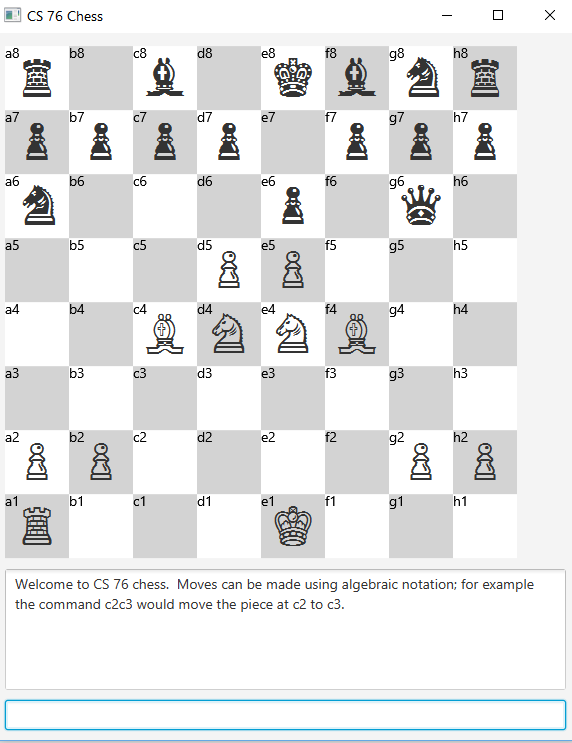
\includegraphics[scale=0.4]{Heuristic1}

\subsection{Material}

The material advantage conceptually works by assuming that the more pieces you have over your opponent, the easier taking more pieces becomes and thus the easier taking the king becomes. Not all pieces are worth the same, however - for example, a queen has much more mobility and threatens many more squares than a pawn does. In order to calculate the material advantage, we assign weights to each of the pieces in accordance to how powerful each piece is considered. This is somewhat arbitrary, but is based on relative values that chess players have used to compare pieces. The values I chose are 100 for a pawn, 340 for a knight, 350 for a bishop, 550 for a rook, and 1000 for a queen. To demonstrate how these values might get used by the AI, since a knight is worth more than 3 times a pawn, the AI might want to lose 3 pawns if it gained them a knight since they would have lost less value than they gained. Another addition to the material advantage is a 100 point bonus if both bishops are still alive - this is because the bishops have distinct areas of threat and can be used in combination to greater effect than twice the value of a single bishop. All the weighted piece values are summed up (only if that piece is still alive) and White's sum is subtracted by Black's sum to get the final material score. 

\subsection{Positional}
The other piece to my evaluation function is the positional advantage. Typically, an actual chess player would factor in many different complicated ideas to determine whether they had a positional advantage, but this takes a significant amount of computational power that is more likely better used in the search. Thus, my evaluation function will have less accuracy when determining the positional advantage than if more attention was paid to these extra factors, but the gain in search depth might be worth that loss. In accordance with this philosophy, I implemented a technique called a piece-square table for each type of piece that gives a score for each square of the board that the piece may be on. These scores don't account for the position of other pieces, so things like pawn formations can't be accurately scored, but general ideas like control of the center or pushing a pawn deeper (towards promotion) can be encouraged. Because these scores depend only on the piece's own position, they can be calculated very quickly. 

This is an example of a piece-square table, for the knight:

\begin{lstlisting}
private static int[][] knightTable = {
	{-40,-30,-25,-20,-20,-25,-30,-40}, //Edges are bad
	{-30,-15, -5,  0,  0, -5,-15,-30},
	{-25, -5,  5, 10, 10,  5, -5,-25},
	{-20,  0, 10, 20, 20, 10,  0,-20}, //Center is good
	{-20,  0, 10, 20, 20, 10,  0,-20},
	{-25, -5,  5, 10, 10,  5, -5,-25},
	{-30,-15, -5,  0,  0, -5,-15,-30},
	{-40,-30,-25,-20,-20,-25,-30,-40}
};
\end{lstlisting}

Basically, positions where the knight has higher mobility (towards the center) give a higher score than those where the knight has lower mobility (especially the corners, where the knight can only make two moves from). The numbers may seem somewhat arbitrary - and yes, they are - but mostly they are based on relative worth. For example, a knight in the center is worth more overall than a bishop on the edges, so the weights should reflect that difference.

\section{Alpha Beta Pruning}

Minimax finds optimal choices, but it is quite slow at doing so and can only search a few depths in a reasonable amount of time. To speed things up, we use alpha-beta pruning to reduce the number of nodes that the algorithm needs to search through. Alpha-beta pruning takes advantage of the alternating minimizing and maximizing that minimax does, and uses scores in previous branches to avoid searching branches that won't have any effect on the outcome of the overall search. Alpha-beta pruning greatly reduces the speed of the search, but has no effect on the results of the search at each depth. To prove this, I tested both searches on the following "Checkmate in 4 moves puzzle":

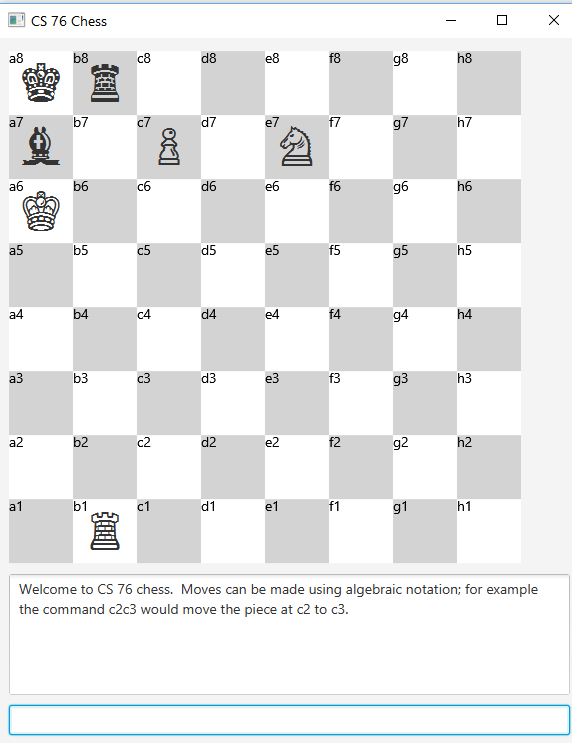
\includegraphics[scale=0.4]{MinimaxTest1}

The solution both algorithms came up with is 1. c7xb8, bxb8 2. nc6 ... 3. rb7 ... 4. ra7++. Note that reproducing this test will have different results if the move ordering and other improvements are included. These results are shown later in the discussion.

The following code shows an addition to the minimax function (maxValue) to use alpha-beta pruning:

\begin{lstlisting}
int result = abMin(newPos, (short) (depth - 1), a, b);
if (result >= b) {
	return b;
}
if (result > a) {
	a = result;
}
\end{lstlisting}

And in minValue:

\begin{lstlisting}
int result = abMax(newPos, (short) (depth - 1), a, b);
if (result <= a) {
	return a;
}
if (result < b) {
	b = result;
}
\end{lstlisting}

As you can see, alpha replaces the "bestValue" in maxValue (now called abMax) and beta replaces the "bestValue" in minValue (now called abMin). A check is added to see if the result is higher than beta (or less than alpha for abMin), and if so, the search breaks off immediately because the final score of the node cannot increase the best path already found.

\section{Transposition Table}

Sometimes, the search will run into the same position twice in the search. Rather than waste time analyzing the same position again, possibly with less accuracy than before, a transposition table is used to store the value that each position was given. If the value stored in the table has a higher depth (meaning more move after that position were analyzed), the score from the table is immediately returned. Otherwise, the position is analyzed like normal and the value in the table is replaced.

\section{Move Ordering Improvements}

Alpha-beta pruning is most effective when the best moves are analyzed first, as more moves get pruned that way. However, when conducting the search, there's no way to know what the best move is, so the "best moves" that are searched first are only guesses. The transposition table stores what the best move was along with the score, so if we've analyzed the same position before, the best move found at a lower depth has a good chance of being the best move at a higher depth, and is thus searched first. 

Another improvement is searching all the capturing moves before the non-capturing moves. Even if capturing a piece isn't the best move, it gives a baseline score and can be calculated quickly, because a capturing move that isn't the best move probably has another capturing move from the other player that punishes it; thus we can start pruning very early on. Of all the extra functionality I implemented, this change actually had the most significant performance increase. For example, on the same checkmate-in-4 puzzle as used before, the modified search finds the solution (at depth 6) of 1. rxb8, bxb8 2.c8->b, ... 3. nc6 ... 4. bb7++ in only about 1,500 milliseconds. In comparison, the typical search finds a checkmate in more than 80,000 milliseconds. It is important to note that the advantage is most likely not always this great, especially in situations with many good non-capturing moves, but I noticed great increases in speed running my algorithm from the typical start of a chess game throughout the entire game - on average, depth 4 takes 2,000 milliseconds to complete, and depth 5 takes about 6,000 milliseconds to complete.


\section{Updated Search}

Including all of the enhancements listed above, this is what a step of my search code looks like. It is largely self explanatory; the previous sections should explain the details of each process.

\begin{lstlisting}
private int abMax(Position position, short depth, int a, int b) {
	if (cutOff(position, depth)) {
		if (!posTable.containsKey(position)) {
			posTable.put(position, new Result(scaling * Heuristic.evaluate(position), depth, (short)-1));
		} 
		return posTable.get(position).score;
	}
	if (posTable.containsKey(position) && posTable.get(position).depth >= depth) {
		return posTable.get(position).score;
	}
	short[] captures = position.getAllCapturingMoves();
	short[] nonCaptures = position.getAllNonCapturingMoves();
	short[] actions = new short[captures.length + nonCaptures.length];
	System.arraycopy(captures, 0, actions, 0, captures.length);
	System.arraycopy(nonCaptures, 0, actions, captures.length, nonCaptures.length);
	//Try to put best move first
	if (posTable.containsKey(position) && posTable.get(position).bestMove != -1) { 
		short guessBestMove = posTable.get(position).bestMove;
		for (int i = 0; i < actions.length; i++) {
			if (actions[i] == guessBestMove) {
				actions[i] = actions[0];
				actions[0] = guessBestMove;
				break;
			}
		}
	}
	short bestMove = actions[0];
	//Iterate through all moves
	for (int i = 0; i < actions.length; i++) {
		try {
			Position newPos = new Position(position);
			newPos.doMove(actions[i]);
			int result = abMin(newPos, (short) (depth - 1), a, b);
			if (result >= b) {
				return b;
			}
			if (result > a) {
				a = result;
				bestMove = actions[i];
			}
		} catch (IllegalMoveException e) {
			System.err.println("Illegal move attempted, this shouldn't be possible.");
			e.printStackTrace();
			System.exit(1);
		}
	}
	posTable.put(position, new Result(a, depth, bestMove));
	return a;
}
\end{lstlisting}

\section{Opening Book}
I added an opening book to my algorithm to help its early game. The AI uses this book by trying to match games in the opening book to the moves it and its opponent have made; if such a match is found, it will make the next move in that match. A few adjustments beyond that have been made; the AI will prioritize winning games, but will take a draw game if it needs to. The AI will give up using the opening entirely if the best game is a loss, because whatever mistakes that player made in their game will carry over to this game as well. I tested using the opening book with a loss and exiting early, hoping to avoid the fatal mistake that player had made and continuing from the mid-game with our own searches, but this still resulted in a positional disadvantage stemming from the actual opening. This strategy would work far better with a larger opening book, as each type of opening would likely have both wins and losses that the AI can use to pick the best move. 

\section{End Game Tables}

Positional advantage in the early and mid game can be quite different than positional advantage in the late game. Notably, the king should be an active participant in pushing the pawns forward rather than hiding in the bottom row. To this end, the heuristic calculates whether we are in the end game using the number of non-pawn/non-king pieces. If there are less than 6 of these pieces, the game is considered in the end-game. This is far from a hard limit, and perhaps an improvement would be a better system for detecting endgame positions, possibly shifting gradually to the end-game positions rather than just activating them on or off. Overall, these end-game tables, while not solving the core problems of the end game AI, do greatly help - before adding them, the AI would choose meaningless actions such as perpetual checks even in the lead, whereas now the AI has a solid goal to work towards.

\end{document}